\chapter{Aan de slag}
\label{ch:aan-de-slag}

In dit hoofdstuk vind je wat technische achtergrond over een aantal onderwerpen die in de labo-opdrachten aan bod kunnen komen. Alles wat hier meegegeven wordt is gebaseerd op jarenlange ervaring, en typische problemen die studenten tegenkomen.

De bedoeling is om een minimum aan informatie mee te geven om je in staat te stellen snel aan de slag te gaan en een aantal typische beginnersfouten te vermijden. Voordat je aan de opdracht begint, lees je dus best eerst de informatie hier na en ga je ook best de \textbf{gerefereerde bronnen opzoeken en bestuderen}!

% TODO:
% Algemene richtlijnen:
% - als je VM helemaal ``om zeep'' gebracht is, doe eenvoudigweg ``vagrant destroy -f; vagrant up'' om opnieuw te beginnen vanaf de laatste werkende versie.
% - wanneer je denkt klaar te zijn met een (deel-)opdracht, genereer de VM nog eens (met destroy en up) en voer alle acceptatietests uit.

\section{Algemene richtlijnen}
\label{sec:algemene_richtlijnen}

In deze sectie vind je enkele algemene richtlijnen die je helpen vlotter en efficiënter te werken.

\begin{itemize}
  \item Open \textbf{verschillende terminalvensters/consoles naast elkaar} (zie Figuur~\ref{fig:screenshot-terminals}). Elke terminal krijgt zijn eigen functie, bijvoorbeeld:
    \begin{itemize}
      \item Vim editor (of Sublime/Notepad/\ldots in een apart venster);
      \item doorvoeren van wijzigingen aan de configuratie;
      \item ingelogd op VM, voor commando's;
      \item ingelogd op VM, voor tonen logbestanden.
    \end{itemize}
  \item \textbf{Werk stap voor stap.} Schrijf niet teveel code ineens. Probeer eerst een minimaal werkende opstelling te verkrijgen en registreer meteen in Git. Maak minimale wijzigingen en \textbf{test elke wijziging uit}. Hoe groter en ingrijpender de wijzigingen, hoe meer kans op fouten en hoe moeilijker die te debuggen zijn. Zodra iets werkt, registreer dit meteen in Git en geef een duidelijke, beschrijvende commit-boodschap.
  \item Suggestie: \textbf{gebruik Git op de command-line.} Bij de meeste Git commando's krijg je gedetailleerde uitleg over hoe je een stap verder moet gaan en ook hoe je de laatste stap kan ongedaan maken. Dit geeft op de duur een beter inzicht in hoe Git precies werkt.
  \item Probeer \textbf{elke commit te beperken tot één enkele ``reden''} om wijzigingen aan te brengen aan de bestaande code. Dit maakt de ``geschiedenis'' van je project transparanter en maakt ook dat je makkelijker kan terugkeren naar een bepaalde stap wanneer je de mist in gaat.
  \item \textbf{Maak backups} van de originele, ongewijzigde configuratiebestanden zodat je er op kan terugvallen als er iets misloopt. Soms heb je zodanig zitten ``prutsen'' dat je er niet meer in slaagt de service te laten werken.
  \item \textbf{Gebruik \texttt{vagrant destroy}} (zie Sectie~\ref{sec:vagrant}). Wanneer je veel manuele wijzigingen hebt aangebracht in een VM, ben je op de duur niet meer zeker dat die zich in de verwachte toestand bevindt. Of je kan door experimenteren de VM onbruikbaar gemaakt hebben. Door de VM te verwijderen en opnieuw op te bouwen (met \texttt{vagrant up}) kan je opnieuw beginnen van een werkende versie (als je de vorige richtlijnen opvolgt, tenminste!).
\end{itemize}

\begin{figure}
  \centering
  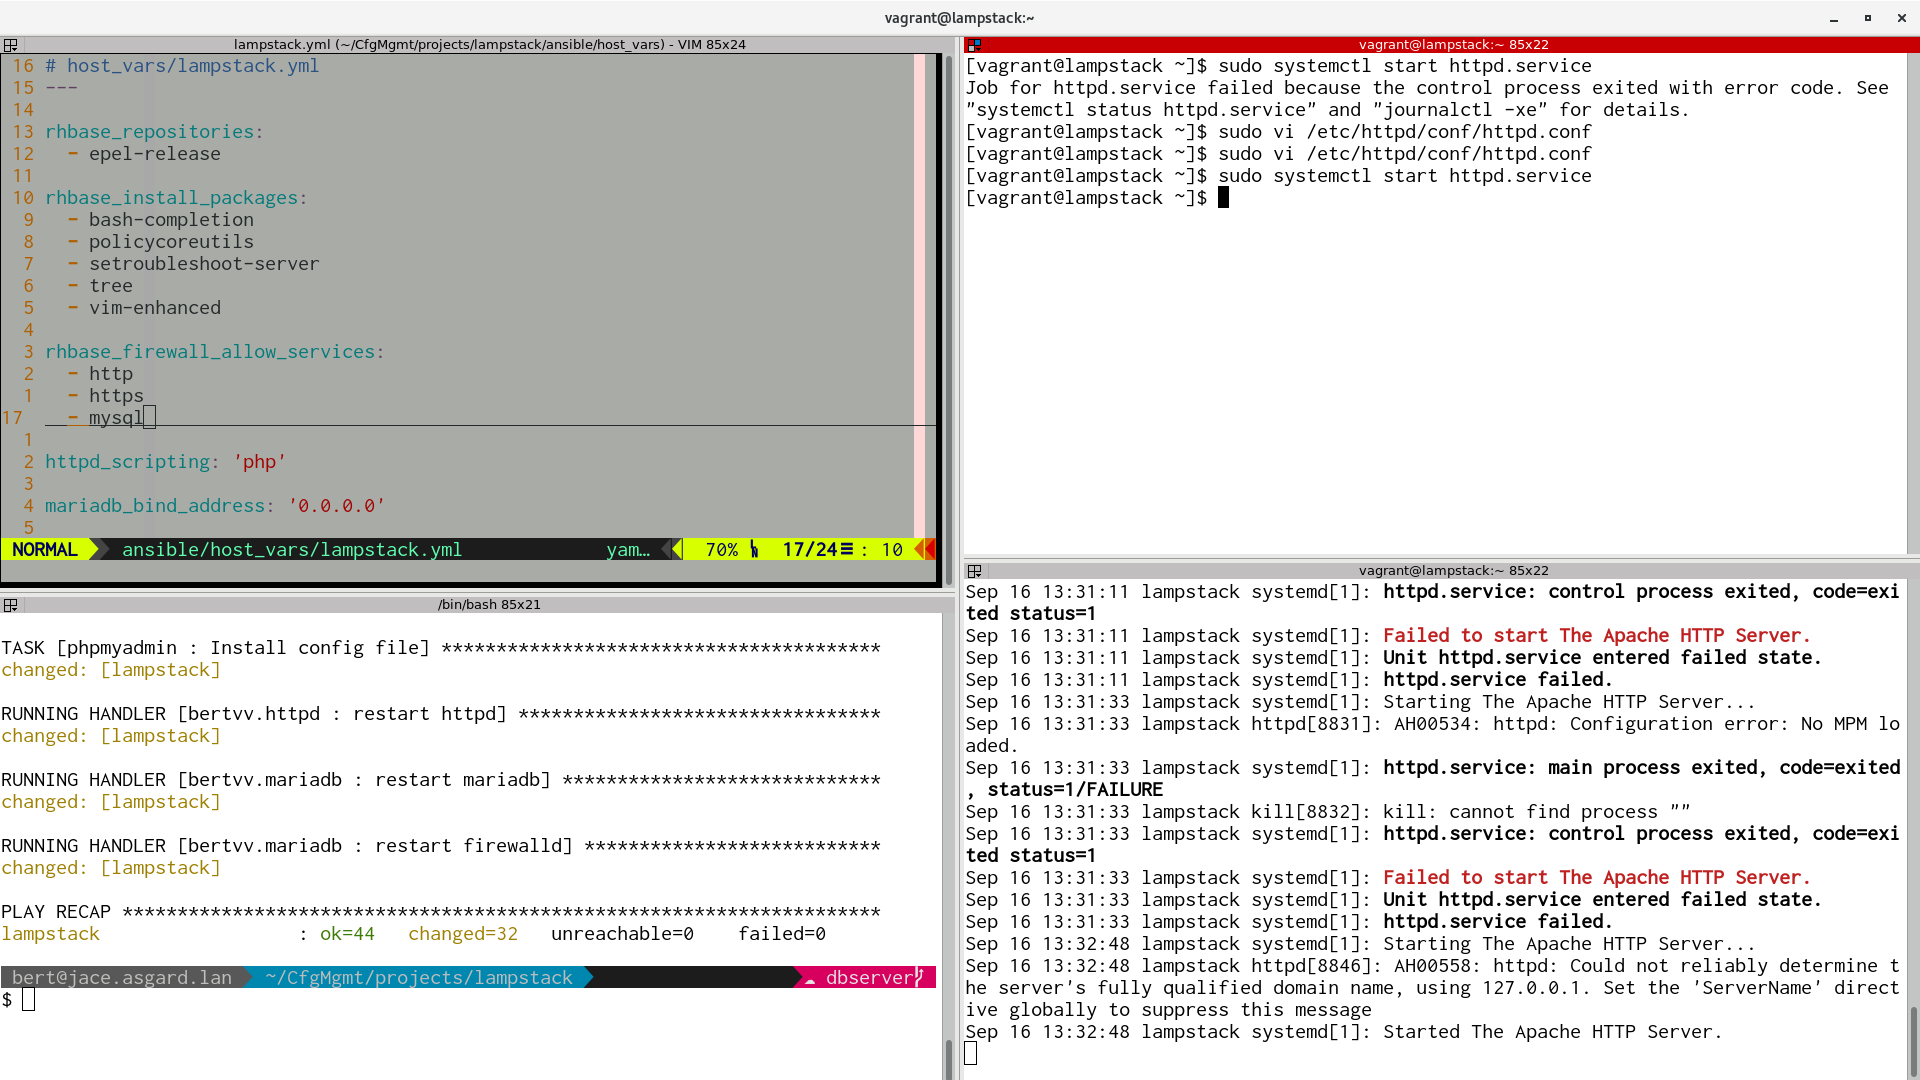
\includegraphics[width=\linewidth]{img/screenshot-terminals}
  \caption[Gebruik van verschillende terminals.]{\textbf{Gebruik van verschillende terminals.} In deze schermafbeelding is Terminator (een terminal-applicatie voor Linux) opgedeeld in vier aparte shells. Linksboven is Vim geopend met een broncodebestand. De terminal linksonder wordt gebruikt om wijzigingen in de broncode door te voeren op de virtuele machines. Rechtsboven is er ingelogd op de virtuele machine waar momenteel wijzigingen op aangebracht worden en kunnen commando's uitgevoerd worden om zaken uit te proberen of problemen op te sporen. Rechtsonder, tenslotte, worden relevante logbestanden van de VM getoond.}
  \label{fig:screenshot-terminals}
\end{figure}

\section{Bash tips}
\label{sec:bash_tips}

In deze sectie vind je een aantal tips voor het gebruik van de Bash-shell. In deze cursus maak je intensief gebruik van de shell, en het loont de moeite om Bash wat beter te leren kennen. Het zit immers vol met interessante features die je toelaten productiever te werken. Online is hier nog veel meer over te vinden~\autocite{Rowe2009}.

De tips hier gelden ook voor Windows- en MacOS-gebruikers! Windows-gebruikers hebben beschikking over een recente versie van Bash via Git (Git Bash). In MacOS X zit ook een Bash-shell, weliswaar een zeer oude versie\footnote{Dit is omwille van de softwarelicentie. Recente versies van Bash vallen onder de open source GPL-licentie, waar Apple niets mee te maken wil hebben.}. Je kan een recente versie installeren via HomeBrew\footnote{\url{http://brew.sh}}.

\begin{itemize}
  \item \textbf{Gebruik \emph{\texttt{TAB}-completion}.} Je kan een deel van een commando of pad intikken en dan de \texttt{TAB}-toets indrukken. Indien mogelijk zal Bash het woord vervolledigen, of mogelijke alternatieven tonen. Als je de package \texttt{bash-completion} installeert zijn er nog veel meer mogelijkheden.
  \item \textbf{Gebruik de \emph{command history}.} Bash houdt de commando's die je eerder gebruikt hebt bij. Met de pijltjestoetsen kan je eerdere commando's terug halen. Gebruik \texttt{Ctrl-R} om te zoeken in de command history. Je kan dan een fragment van het commando intikken, Bash toont dan het laatste commando waar dat tekstfragment in voorkomt.
  \item \textbf{Bang bang!} In Bash zijn er enkele shortcuts voorzien voor (delen van) het vorige commando. \texttt{!!} staat voor het gehele vorige commando, \texttt{!\$} voor het laatste argument en \texttt{!*} voor alle argumenten. Een voorbeeldje van het gebruik:

    \begin{minted}{console}
$ yum update
You need to be root to perform this command.
$ sudo !!
sudo yum update
[...]
$ mkdir -p some/long/path/i/dont/want/to/repeat
$ cd !$
cd some/long/path/i/dont/want/to/repeat
$
\end{minted}
  \item \textbf{Toetsenbordcombinaties.} Naast \texttt{Ctrl-R} van hierboven zijn er nog een aantal nuttige toetsenbordcombinaties.
    \begin{itemize}
      \item \texttt{Ctrl-C} onderbreekt het huidige proces
      \item \texttt{Ctrl-Z} pauzeert het huidige proces (haal het terug met \texttt{fg})
      \item \texttt{Ctrl-D} sluit de shell af (enkel op lege regel)
      \item \texttt{Ctrl-K} verwijdert de tekst rechts van de cursor
      \item \texttt{Ctrl-U} verwijdert de tekst links van de cursor
      \item \texttt{Ctrl-T} verwisselt letterteken onder de cursor met dat voor de cursor
      \item \texttt{Alt-T} verwisselt woord voor met woord na de cursor
    \end{itemize}

    Er bestaan nog \emph{veel} meer combinaties. Deze kan je vinden in de man-pagina \texttt{bash(1)} in de sectie READLINE (subsectie \emph{Readline Command Names} en volgende).

  \item \textbf{Personaliseer de shell.} Je kan het gedrag van de shell in hoge mate aan je eigen wensen aanpassen door het bestand \path{~/.bashrc}\footnote{Het symbool {\textasciitilde} is natuurlijk de \emph{home directory} van de gebruiker. In Linux komt dit overeen met \path{/home/USER}, onder Windows met \path{C:\Users\USER} of \path{C:\Gebruikers\USER}, onder MacOS met \path{/Users/USER}} aan te passen. Je kan het gedrag van tab-completion of de command history aanpassen, een eigen commandoprompt instellen, aliassen (zie verder) of functies definiëren, enz. Het zou ons te ver leiden om alle mogelijkheden uit te diepen, maar je kan een uitgebreid voorbeeld vinden in \url{https://github.com/bertvv/dotfiles/} (of gelijknamige repositories van andere Github-gebruikers).

  \item \textbf{Aliassen} zijn een soort shortcuts voor commando's die je vaak gebruikt. Dit kan enorm veel typwerk besparen. Je kan ze toevoegen in je \path{~/.bashrc}. Enkele voorbeelden:

    \begin{minted}{bash}
alias l='ls -l --si --time-style=long-iso --color'
alias a='git add'
alias c='git commit -m'
alias h='git log --pretty="format:%C(yellow)%h %C(blue)%ad %C(reset)%sC(red)%d %C(green)%an%C(reset), %C(cyan)%ar" --date=short --graph --all'
alias s='git status'
alias vu='vagrant up'
alias vD='vagrant destroy'
\end{minted}

    Nog meer voorbeelden vind je in \url{https://github.com/bertvv/dotfiles/blob/master/.bash.d/aliases.sh}.
\end{itemize}

\section{Vagrant}
\label{sec:vagrant}

Vagrant is een command line tool die het aanmaken en configureren van virtuele machines automatiseert. Het ondersteunt een aantal virtualisatieplatforms, o.a.~VirtualBox, Hyper-V, libvirt, enz. Wij zullen het gebruiken in combinatie met VirtualBox. Voor een demo van de werking van Vagrant, bekijk eerst de screencast van \textcite{Weissig2014}.

Je Git repository bevat een Vagrant-omgeving voor het opzetten van de VMs voor je labo-opdracht. Er is alvast één VM gedefinieerd.  Je kan een overzicht van de VMs opvragen met (voorbeeld uit de SME-opdracht van Sectie~\ref{subs:smallmedium-enterprise-infrastructure}):

\begin{minted}{console}
$ vagrant status
Current machine states:

pu004                     not created (virtualbox)

The environment has not yet been created. Run `vagrant up` to
create the environment. If a machine is not created, only the
default provider will be shown. So if a provider is not listed,
then the machine is not created for that environment.
$
\end{minted}

De hostnaam \texttt{pu004} slaat op het feit dat deze host in een publiek toegankelijk zit. Het getal is een volgnummer dat verder geen betekenis heeft. Hosts in een privaat netwerk dat niet van buitenaf toegankelijk is, zouden beginnen met \texttt{pr} gevolgd door een nummer (bv. \texttt{pr002}). Goede namen geven aan servers is niet altijd makkelijk en er bestaan verschillende benaderingen~\autocite{Mytton2015,mnxio}. De gekozen opgave legt de servernamen op, of geeft aanwijzingen.

Start de VM met \texttt{vagrant\ up}. De eerste keer dat je dit doet wordt er een basis-VM gedownload met een minimale installatie van de laatste stabiele versie van CentOS. Die zal telkens dienst doen als basis voor het opzetten van alle hosts in ons netwerk.

Na opstarten kan je inloggen met \texttt{vagrant\ ssh\ pu004}. Je bent ingelogd als gebruiker \texttt{vagrant} en kan commando's uitvoeren met \texttt{root}-rechten door er \texttt{sudo} voor te plaatsen (geen wachtwoord vereist). Als het nodig mocht zijn: het wachtwoord van de gebruikers \texttt{vagrant} en \texttt{root} is telkens \texttt{vagrant}.

Als je \texttt{ls\ /} uitvoert, zal je merken dat er een directory \path{/vagrant} bestaat. Dit is je lokale repository die gemount is binnen de VM. Dit is een eenvoudige manier om bestanden te delen tussen VM en host-systeem.

Let er op dat je VMs niet meer vanuit je VirtualBox GUI opstart of bewerkt. Doe dit nu enkel met Vagrant en vanuit een terminal. Het commando \texttt{vagrant} moet altijd uitgevoerd worden vanuit de directory waar het bestand \texttt{Vagrantfile} zich bevindt.

De belangrijkste Vagrant commando's worden opgesomd in Tabel~\ref{tab:vagrant-commandos}. Daar waar \texttt{[VM]} tussen rechte haken staat, is dat een optioneel argument. Als je het weglaat, wordt de actie op \emph{alle} VMs tegelijk uitgevoerd.

\begin{longtable}{@{}ll@{}}
  \toprule
  Commando & Functie\tabularnewline
  \midrule
  \endhead
  \texttt{vagrant\ status} & Geef een overzicht van de Vagrant-omgeving\tabularnewline
  \texttt{vagrant\ up\ [VM]} & Start \texttt{VM} op\tabularnewline
  \texttt{vagrant\ provision\ [VM]} & Draai het configuratiescript op \texttt{VM}\tabularnewline
  \texttt{vagrant\ ssh\ VM} & Log in op \texttt{VM} als gebruiker \texttt{vagrant}\tabularnewline
  \texttt{vagrant\ halt\ [VM]} & Stop \texttt{VM}\tabularnewline
  \texttt{vagrant\ reload\ [VM]} & Herstart \texttt{VM}\tabularnewline
  \texttt{vagrant\ destroy\ [VM]} & Vernietig \texttt{VM}\tabularnewline
  \bottomrule
\caption{De belangrijkste \texttt{vagrant}-commando's}
\label{tab:vagrant-commandos}
\end{longtable}

\section{Ansible}
\label{sec:ansible}

Ansible is een \emph{configuration management system,} d.w.z. het staat in voor het configureren van een host vanaf een minimale installatie tot een volledig operationeel systeem. Het concept van een configuration management tool is dat je beschrijft wat de gewenste toestand van het systeem is, de tool zorgt er voor dat het systeem in die toestand terecht komt. Bekijk de screencast van \textcite{Weissig2015} voor een inleiding op Ansible. In een vervolg-screencast wordt ook de combinatie van Ansible en Vagrant belicht. In deze gids geven we enkel wat uitleg om aan de slag te gaan met de startopstelling voor de labo-opdracht, maar als je op zoek bent naar een goed naslagwerk over Ansible, overweeg dan om het e-boek van \textcite{Geerling2016} te kopen. De auteur werkt nog verder aan het boek, updates zijn gratis.

Sommige config management systemen hebben een eigen taal ontwikkeld om die configuratie in te beschrijven (bv. Puppet), andere gebruiken een bestaande taal (bv. Chef, configuratie in Ruby). Bij Ansible beschrijf je de configuratie van een systeem met Yaml, een eenvoudig tekstformaat om data te structureren op een manier die makkelijk te interpreteren is zowel door mensen als computers. De bestanden die deze configuratiecode bevatten worden \emph{playbooks}\footnote{\url{https://docs.ansible.com/ansible/playbooks.html}} genoemd. Als je deze playbooks op een specifieke manier structureert en herbruikbaar maakt, spreekt men van een \emph{rol}\footnote{\url{https://docs.ansible.com/ansible/playbooks_roles.html\#roles}}. Je kan rollen toekennen aan een host, en specifieke instellingen toepassen door het invullen van \emph{variabelen}\footnote{\url{https://docs.ansible.com/ansible/playbooks_variables.html}}. Op Ansible Galaxy\footnote{\url{https://galaxy.ansible.com/}} kan je tientallen rollen vinden die door hun auteurs gepubliceerd zijn.

De directorystructuur van een Ansible-project ligt vast en wordt uitvoerig beschreven in de documentatie\footnote{\url{https://docs.ansible.com/ansible/playbooks_best_practices.html}}.

\subsection{Rollen toekennen aan hosts}
\label{sub:rollen-toekennen-aan-hosts}

Om een rol toe te kennen aan een host, bewerk je de \emph{master playbook} \path{ansible/site.yml}. Dit bestand bevat een overzicht van alle hosts onder het beheer van Ansible, met de rollen van elke host:

\begin{minted}{yaml}
# site.yml
---
- hosts: pu004
  sudo: true
  roles: []
\end{minted}

Host \texttt{pu004} heeft nog geen rollen toegekend, dat gaan we nu veranderen:

\begin{minted}{yaml}
# site.yml
---
- hosts: pu004
  sudo: true
  roles:
    - bertvv.rh-base
\end{minted}

Onder \texttt{roles:} kan je zoveel rollen toevoegen als nodig. Let goed op de indentatie. Je \textbf{moet} telkens inspringen met 2 spaties, en alle data op hetzelfde niveau moet links mooi uitgelijnd zijn.

\subsection{Rollen installeren}
\label{sub:rollen-installeren}

Alle rollen die gebruikt worden in \path{site.yml} moeten beschikbaar zijn in de directory \path{ansible/roles/} in een subdirectory met dezelfde naam als deze gebruikt in \path{site.yml}.

De naam van de rol \path{bertvv.rh-base} is geschreven in de vorm \path{AUTEUR.ROLNAAM}. Dit wijst er op dat deze rol op Ansible Galaxy gepubliceerd is. Je kan die daar terugvinden onder de url ``\url{http://galaxy.ansible.com/AUTEUR/ROLNAAM/}.'' Je kan daar de rol downloaden en uitpakken op de juiste plaats in de Ansible-directorystructuur.

Dit is het eenvoudigste als je MacOS of Linux op je hostsysteem draait. Je kan dan Ansible installeren en gebruik maken van het commando \texttt{ansible-galaxy}:

\begin{minted}{console}
$ ansible-galaxy -p ansible/roles install bertvv.httpd
- downloading role 'httpd', owned by bertvv
- downloading role from https://github.com/bertvv/ansible-role-httpd/archive/v1.2.1.tar.gz
- extracting bertvv.httpd to ansible/roles/bertvv.httpd
- bertvv.httpd was installed successfully
$
\end{minted}

Dit commando zal de rol \path{bertvv.rh-base} downloaden en uitpakken onder directory \path{ansible/roles}.

Onder Windows wordt Ansible niet ondersteund, en is dit commando dus ook niet beschikbaar. Je kan wel manueel een rol downloaden van de Github-repository (bijvoorbeeld voor \path{bertvv.rh-base} van \url{https://github.com/bertvv/ansible-role-rh-base/releases}) en dan op de juiste plaats uitpakken.

In je repository is ook een scriptje voorzien dat het installatieproces automatiseert: \path{scripts/role-deps.sh}. Als je het uitvoert in een Bash shell vanuit de hoofddirectory van je repository, zal het in \path{ansible/site.yml} alle rollen die er vernoemd worden van Ansible Galaxy (of indien de rol daar niet gepubliceerd is van Github) downloaden en installeren. Dit script werkt trouwens ook op MacOS en Linux.

Merk op dat rollen van Ansible Galaxy genegeerd worden door Git. Het heeft geen zin je eigen repository te ``vervuilen'' met code die al elders onderhouden wordt. Het is dus ook de bedoeling dat je \emph{geen wijzigingen} aanbrengt in bestaande rollen. Als dit toch nodig is (omdat er bv. features ontbreken die je zelf geïmplementeerd hebt), is het beter de oorspronkelijke rol te ``forken'' op Github en daar te onderhouden.

Na installatie van de rollen, kan je met \texttt{vagrant\ provision} de \emph{master playbook} uitvoeren.

\subsection{Hosts configureren}
\label{sub:hosts-configureren}

Als je de documentatie voor een rol naleest (typisch het bestand README.md van de Github repository), vind je in principe een lijst met \emph{rolvariabelen} die je kan invullen voor het toepassen van concrete instellingen voor hetzij specifieke hosts, hetzij groepen van hosts. Variabelen die voor \emph{alle} hosts gelden, moeten gedefinieerd worden in het bestand \path{ansible/group_vars/all.yml}. Variabelen voor specifieke hosts in \path{ansible/host_vars/HOSTNAAM.yml}. Het formaat is opnieuw Yaml, en de structuur van zo'n bestand is zeer eenvoudig. Je geeft een opsomming van variabelen met de waarde die je er aan wil geven. Een voorbeeld:

\begin{minted}{yaml}
---
rhbase_repositories:
  - epel-release
rhbase_install_packages:
  - bash-completion
  - vim-enhanced
rhbase_firewall_allow_services
  - http
  - https
\end{minted}

Telkens je een wijziging aanbrengt in de Ansible-configuratie, kan je die doorvoeren met \texttt{vagrant\ provision}.


% TODO:
% Sectie over basiskennis CentOS
% (na Ansible)


\section{DNS en BIND}
\label{sec:dns-en-bind}

% TODO: verwijs naar het rocket scientists boek

DNS is essentieel voor de correcte werking van een domein, en redelijk wat (volgens sommigen \emph{alle}\footnote{\url{http://www.krisbuytaert.be/blog/}}) netwerkproblemen zijn terug te leiden tot fouten in DNS. Er zijn verschillende implementaties van DNS, maar veruit de meest gebruikte (en dus essentieel voor de werking van het Internet als geheel) is BIND\footnote{\url{https://www.isc.org/downloads/bind/}}.

DNS is op zich geen complexe netwerkservice. Het komt neer op een databank met enkele tabellen (= zonebestanden) die in (een strak) tekstformaat zijn opgemaakt. Er zijn verschillende types van records, o.a.

\begin{itemize}
\item \texttt{A} bevat het IPv4-adres voor een gegeven hostnaam;
\item \texttt{AAAA} idem, maar voor IPv6;
\item \texttt{CNAME} bevat de ``originele'' hostnaam voor een gegeven alias (kan bijvoorbeeld worden gebruikt voor ``www.linuxlab.lan'');
\item \texttt{MX} bevat verwijzingen naar de mailservers voor dit domein;
\item \texttt{NS} bevat verwijzingen naar de DNS-servers voor dit domein;
\item \texttt{PTR} bevat de hostnaam voor een gegeven IP-adres (bevindt zich normaal in een zgn.\emph{reverse lookup} zonebestand);
\item enz. (lees de documentatie!)
\end{itemize}

Een zonebestand begint met een zgn. SOA-record, wat staat voor Start Of Authority. Hieronder vind je een voorbeeld van een \emph{forward zone file} voor een domein met de naam ``linuxlab.lan'' voor het IPv4-netwerk 192.168.15.0/24. Op de precieze betekenis gaan we hier niet in, dit wordt elders voldoende uitgediept~\autocite{Aitchison2015}.

\begin{verbatim}
; /var/named/linuxlab.lan
; Forward lookup zone file for `linuxlab.lan.'
$ORIGIN linuxlab.lan.
$TTL 1W
;        primary DNS   email address admin
@ IN SOA srv001        hostmaster (
   2015101216   ; serial
   1D           ; refresh
   1H           ; retry
   1W           ; expire
   1D           ; minimum TTL
)
\end{verbatim}

De overeenkomstige \emph{reverse zone file} begint als volgt:

\begin{verbatim}
; /var/named/15.168.192.in-addr.arpa.
; Reverse lookup zone file for `linuxlab.lan.'
$ORIGIN 15.168.192.in-addr.arpa.
$TTL 1W
@ IN SOA srv001.linuxlab.lan. hostmaster.linuxlab.lan. (
   2015101216   ; serial
   1D           ; refresh
   1H           ; retry
   1W           ; expire
   1D           ; minimum TTL
)
\end{verbatim}

De syntax van deze \emph{zone files} is heel strak en het is makkelijk om fouten te maken. De meest voorkomende fouten zijn de volgende:

\begin{itemize}
  \item Hostnamen die volledig uitgeschreven zijn (\emph{ully qualified domain name} of FQDN) moeten in een zonebestand altijd afgesloten worden met een punt, bv. ``\texttt{pu001.linuxlab.net.}''. Namen die niet op een punt eindigen, worden aangevuld met de waarde van \texttt{\$ORIGIN} die aan het begin van een zonebestand gegeven wordt (d.i. de domeinnaam, in ons geval ``\texttt{linuxlab.net.}''). Bv.  \texttt{pu002} wordt dan ``\texttt{pu002.linuxlab.net.}''. Als je een hostnaam volledig uitschrijft en je vergeet de punt, dan zal de domeinnaam dus verkeerd geïnterpreteerd worden. ``\texttt{pu002.linuxlab.net}'' wordt immers omgezet naar ``\path{pu002.linuxlab.net.linuxlab.net.}''.
\item IP-adressen worden op een eigenaardige manier genoteerd. Ten eerste wordt het host-deel van het netwerkadres niet geschreven, de getallen in de ``dotted quad''-notatie worden omgekeerd en je moet er ``\texttt{in-addr.arpa.}'' achter schrijven. Met andere woorden, \texttt{192.0.2.0/24} wordt als ``\texttt{2.0.192.in-addr-arpa."} geschreven.
\end{itemize}

Het is niet altijd evident om fouten op te sporen in de configuratie van een BIND DNS-server. Daarom deze tips:

\begin{itemize}
  \item Test de syntax van configuratiebestanden voordat je de service opstart. Voor het hoofd-configuratiebestand \path{/etc/named.conf} is het commando:
    \begin{verbatim}
$ sudo named-checkconf /etc/named.conf
    \end{verbatim}
  \item De syntax testen van zonebestanden gebeurt zo (voorbeeld voor forward en reverse zone, respectievelijk):

    \begin{verbatim}
$ sudo named-checkzone linuxlab.lan /var/named/linuxlab.lan
$ sudo named-checkzone 15.168.192.in-addr.arpa \
    /var/named/15.168.192.in-addr.arpa
    \end{verbatim}

\item Je kan foutboodschappen van de service bekijken met \texttt{journalctl}. Het handigste is om een aparte console te openen, in te loggen op je server en dan het volgende commando uit te voeren:

    \begin{verbatim}
$ sudo journalctl -l -f -u named.service
    \end{verbatim}

  Open een andere console om commando's uit te voeren (bv. de service herstarten). Je ziet dan meteen relevante info- en foutboodschappen verschijnen.
\end{itemize}

\section{Fileservers en Samba}
\label{sec:fileservers-en-samba}

De meest gebruikte manier om met Linux een fileserver op te zetten die voor alle desktop-operating systems beschikbaar is, is met Samba. Het Samba-project heeft al een lange geschiedenis achter de rug en is eigenlijk een onafhankelijke implementatie van het SMB-protocol dat je misschien beter kent als Windows Network Neighbourhood.

De laatste versie van Samba laat zelfs toe als een Active Directory Domain Controller op te treden, maar dat valt buiten het bestek van deze cursus.

Het opzetten van een Samba fileserver is soms een uitdaging, vooral wat betreft het juist instellen van de toegangsrechten. Als je bepaalde gebruikers wil lees- of schrijftoegang geven tot een share, dan moet dit op drie verschillende niveaus correct ingesteld zijn:

\begin{enumerate}
\def\labelenumi{\arabic{enumi}.}
\item \textbf{Bestandspermissies:} De gewone bestandspermissies moeten de gebruiker lees- of schrijftoegang geven.
\item \textbf{Samba configuratie:} De share moet via het Samba-configuratiebestand \path{/etc/samba/smb.conf} de juiste toegangsrechten toekennen aan de gebruiker
\item \textbf{SELinux:} De directory moet de juiste SELinux context hebben (zie RedHat manual)
\end{enumerate}

Als ook maar één van deze drie elementen te streng is ingesteld, hebben de gebruikers niet de gewenste toegang. Door dit proces te automatiseren, kan je vervelende fouten (en de tijd die nodig is die op te lossen) vermijden.

Samba voorziet een commando voor het controleren of het configuratiebestand \path{/etc/samba/smb.conf} correct is: \texttt{testparm}. Het drukt ook de inhoud van het configuratiebestand af in de meest eenvoudige en compacte vorm. Dit kan ook van pas komen om de configuratie die je zelf hebt opgebouwd te ``optimaliseren''. Samba voorziet namelijk standaardinstellingen die je niet moet expliciet schrijven (bijvoorbeeld \texttt{guest\ ok\ =\ no}) en er zijn ook vaak verschillende manieren om hetzelfde te schrijven (bijvoorbeeld \texttt{guest\ ok\ =\ no} is het zelfde als \texttt{public\ =\ yes}). Sommige opties worden zelfs genegeerd afhankelijk van de waarde van andere (bijvoorbeeld \texttt{guest\ only} heeft geen effect als \texttt{guest\ ok} niet is ingesteld). Geef de optie \texttt{-s} of \texttt{-\/-suppress-prompt} mee, om te vermijden dat er gevraagd wordt om ``ENTER'' in te drukken voordat je het overzicht van de configuratie te zien krijgt.

Om te testen of de share toegankelijk is van buitenaf, kan je vanop het hostsysteem in de file explorer werken, maar dit is niet zo interessant.  De foutboodschappen geven weinig of geen informatie die helpt bij het vinden van de oorzaak van het probleem. Gebruik liever \texttt{smbclient}, daarmee krijg je alvast iets duidelijker foutboodschappen. Enkele voorbeelden van het gebruik:

\begin{verbatim}
## Geef een overzicht van de shares op server FILES
smbclient -L //files/

## Log in op een share als gebruiker lizae met wachtwoord letmein
smbclient //files/public/ -Ulizae%letmein

## Log in op een share als "gast"
smbclient //files/public -U%
\end{verbatim}

\section{Troubleshooting}
\label{sec:troubleshooting-1}

Het gebruik maken van een configuration management system laat een systeembeheerder toe om op een gecontroleerde en betrouwbare manier snel netwerkservices in productie te brengen. Het configuration management system vereenvoudigt het opzetten van een service en door de doorgedreven automatisering worden fouten tot een minimum beperkt.

Jammer genoeg ontslaat dit ons niet van de verantwoordelijkheid om de systemen die we beheren van binnen en van buiten te kennen en de interne werking te begrijpen. Wanneer er toch fouten de kop op steken en onze systemen zijn niet beschikbaar voor onze gebruikers, brengt het configuration managementsysteem niet altijd soelaas. Integendeel, op dat moment is het niet meer dan een extra laag complexiteit.

Een systematische en grondige aanpak is van levensbelang. De impact van de onbeschikbaarheid van netwerkservices is meestal bijzonder zwaar. In het beste geval heb je boze gebruikers, maar in het slechtste geval verliest je bedrijf tienduizenden euro's per uur aan verloren productiviteit en potentiële inkomsten. Op zo'n moment gaat met googlen naar een oplossing kostbare tijd verloren (als je al \emph{kan} googlen), en als je op dat moment nog moet beginnen handleidingen lezen, wordt het zeker nachtwerk.

% TODO: aanvullen, verwijzen naar network troubleshooting guide
